\chapter{Anexo: Telegramas}

\section{Ejemplo de telegrama}
\label{anexo:telegrama}

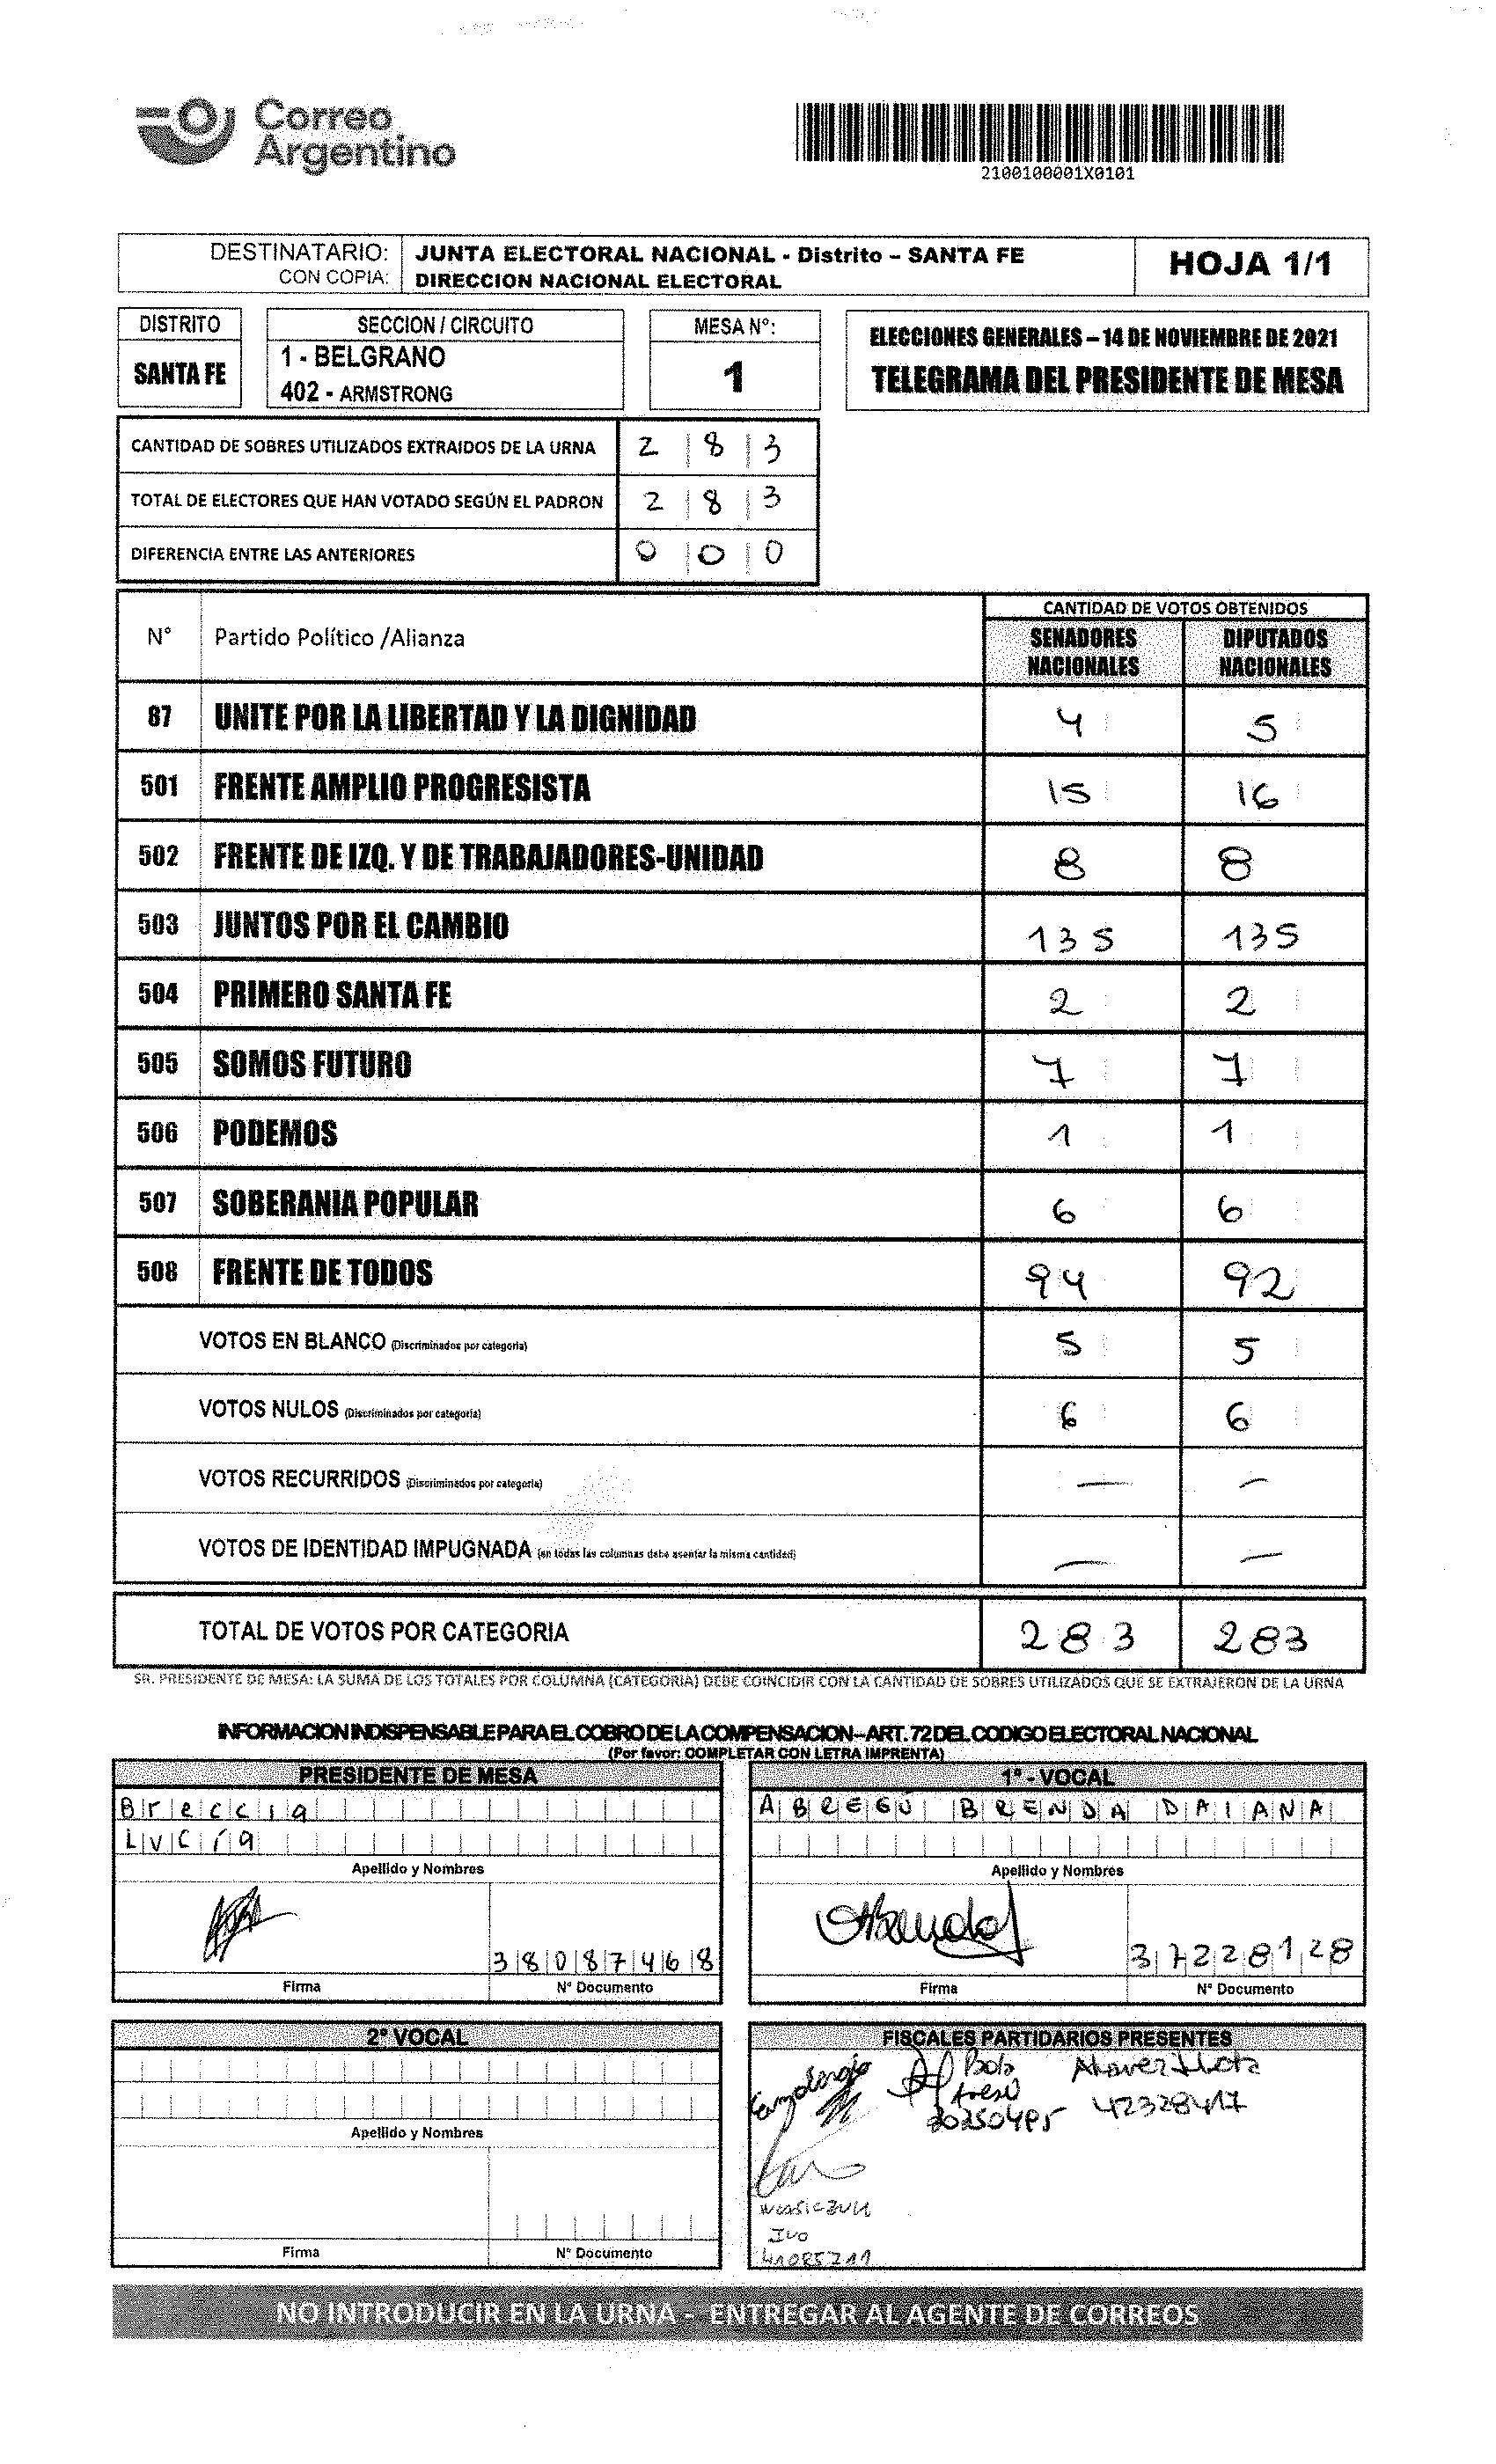
\includegraphics[height=0.8\textheight]{appendices/telegrama.jpg}

\section{Ejemplo de telegrama mal cargado}
\label{anexo:telegrama-erroneo}

El telegrama cargado corresponde a elecciones de concejales locales en vez de diputados o senadores nacionales.

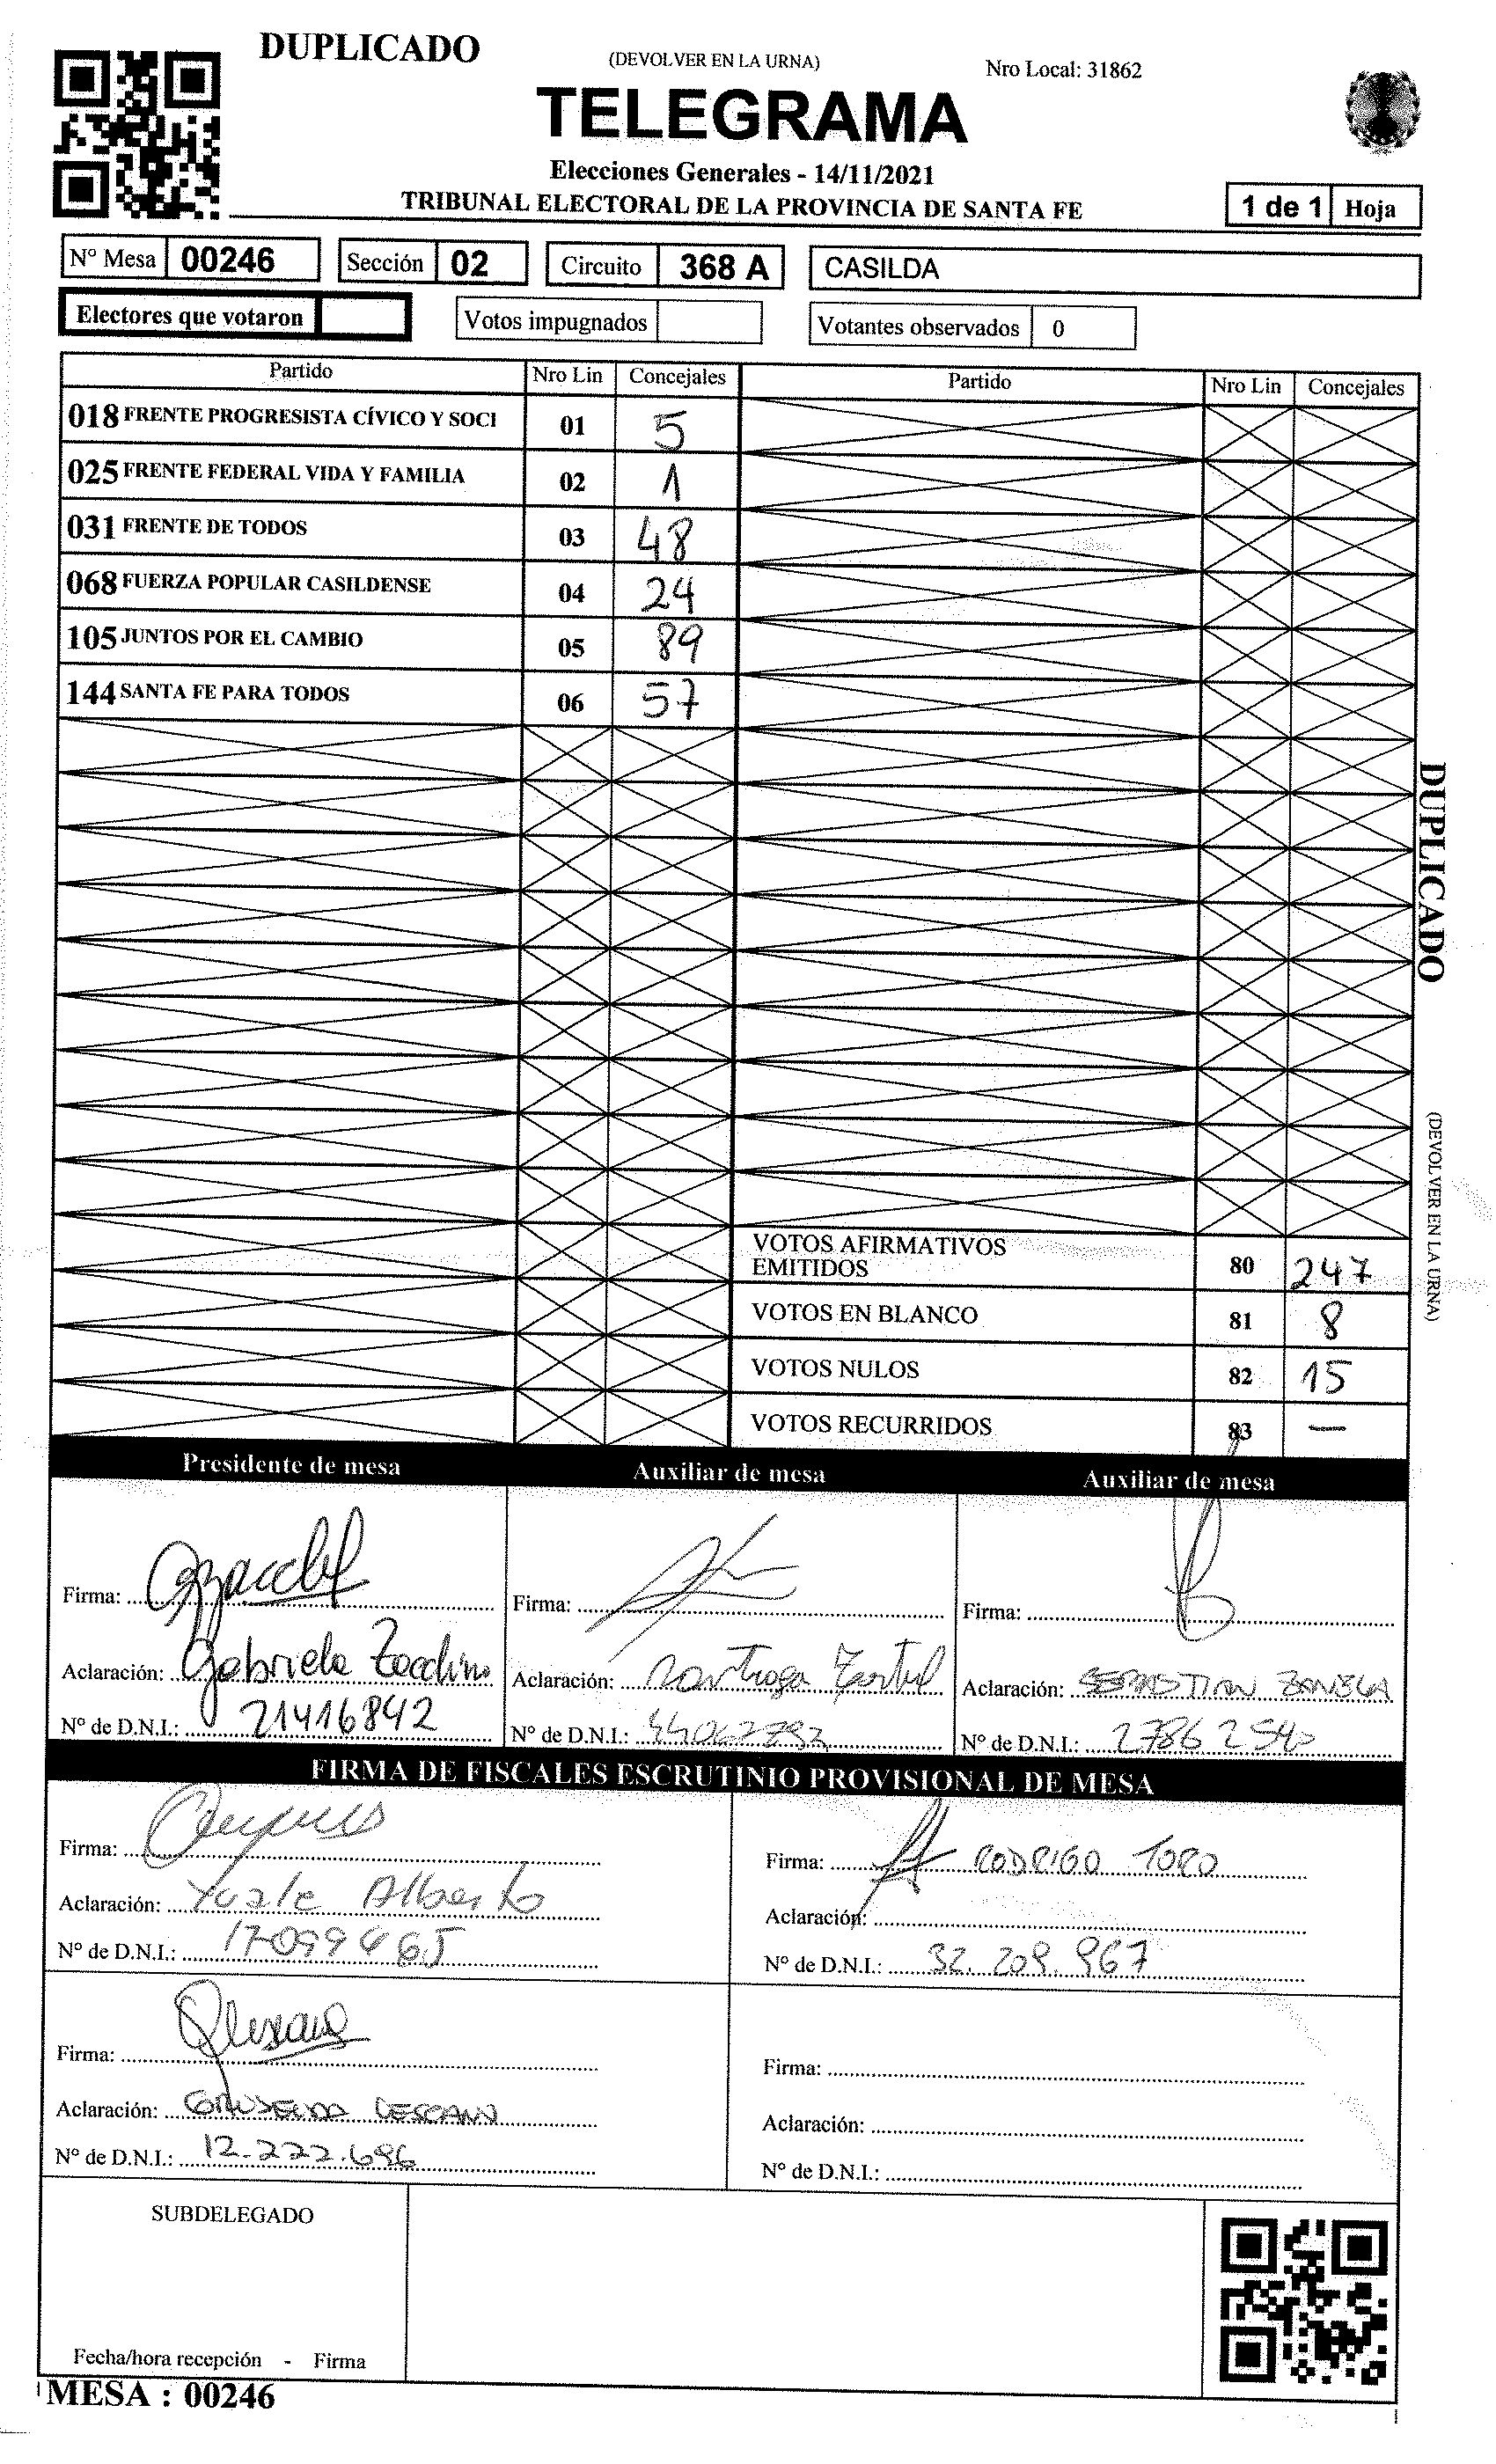
\includegraphics[height=0.8\textheight]{appendices/telegrama-erroneo.jpg}

\section{Ejemplo de telegrama con números sin espacio entre ellos}
\label{anexo:telegrama-numeros-juntos}

El telegrama no posee espacios entre los números, por lo que resulta complicado segmentarlos.

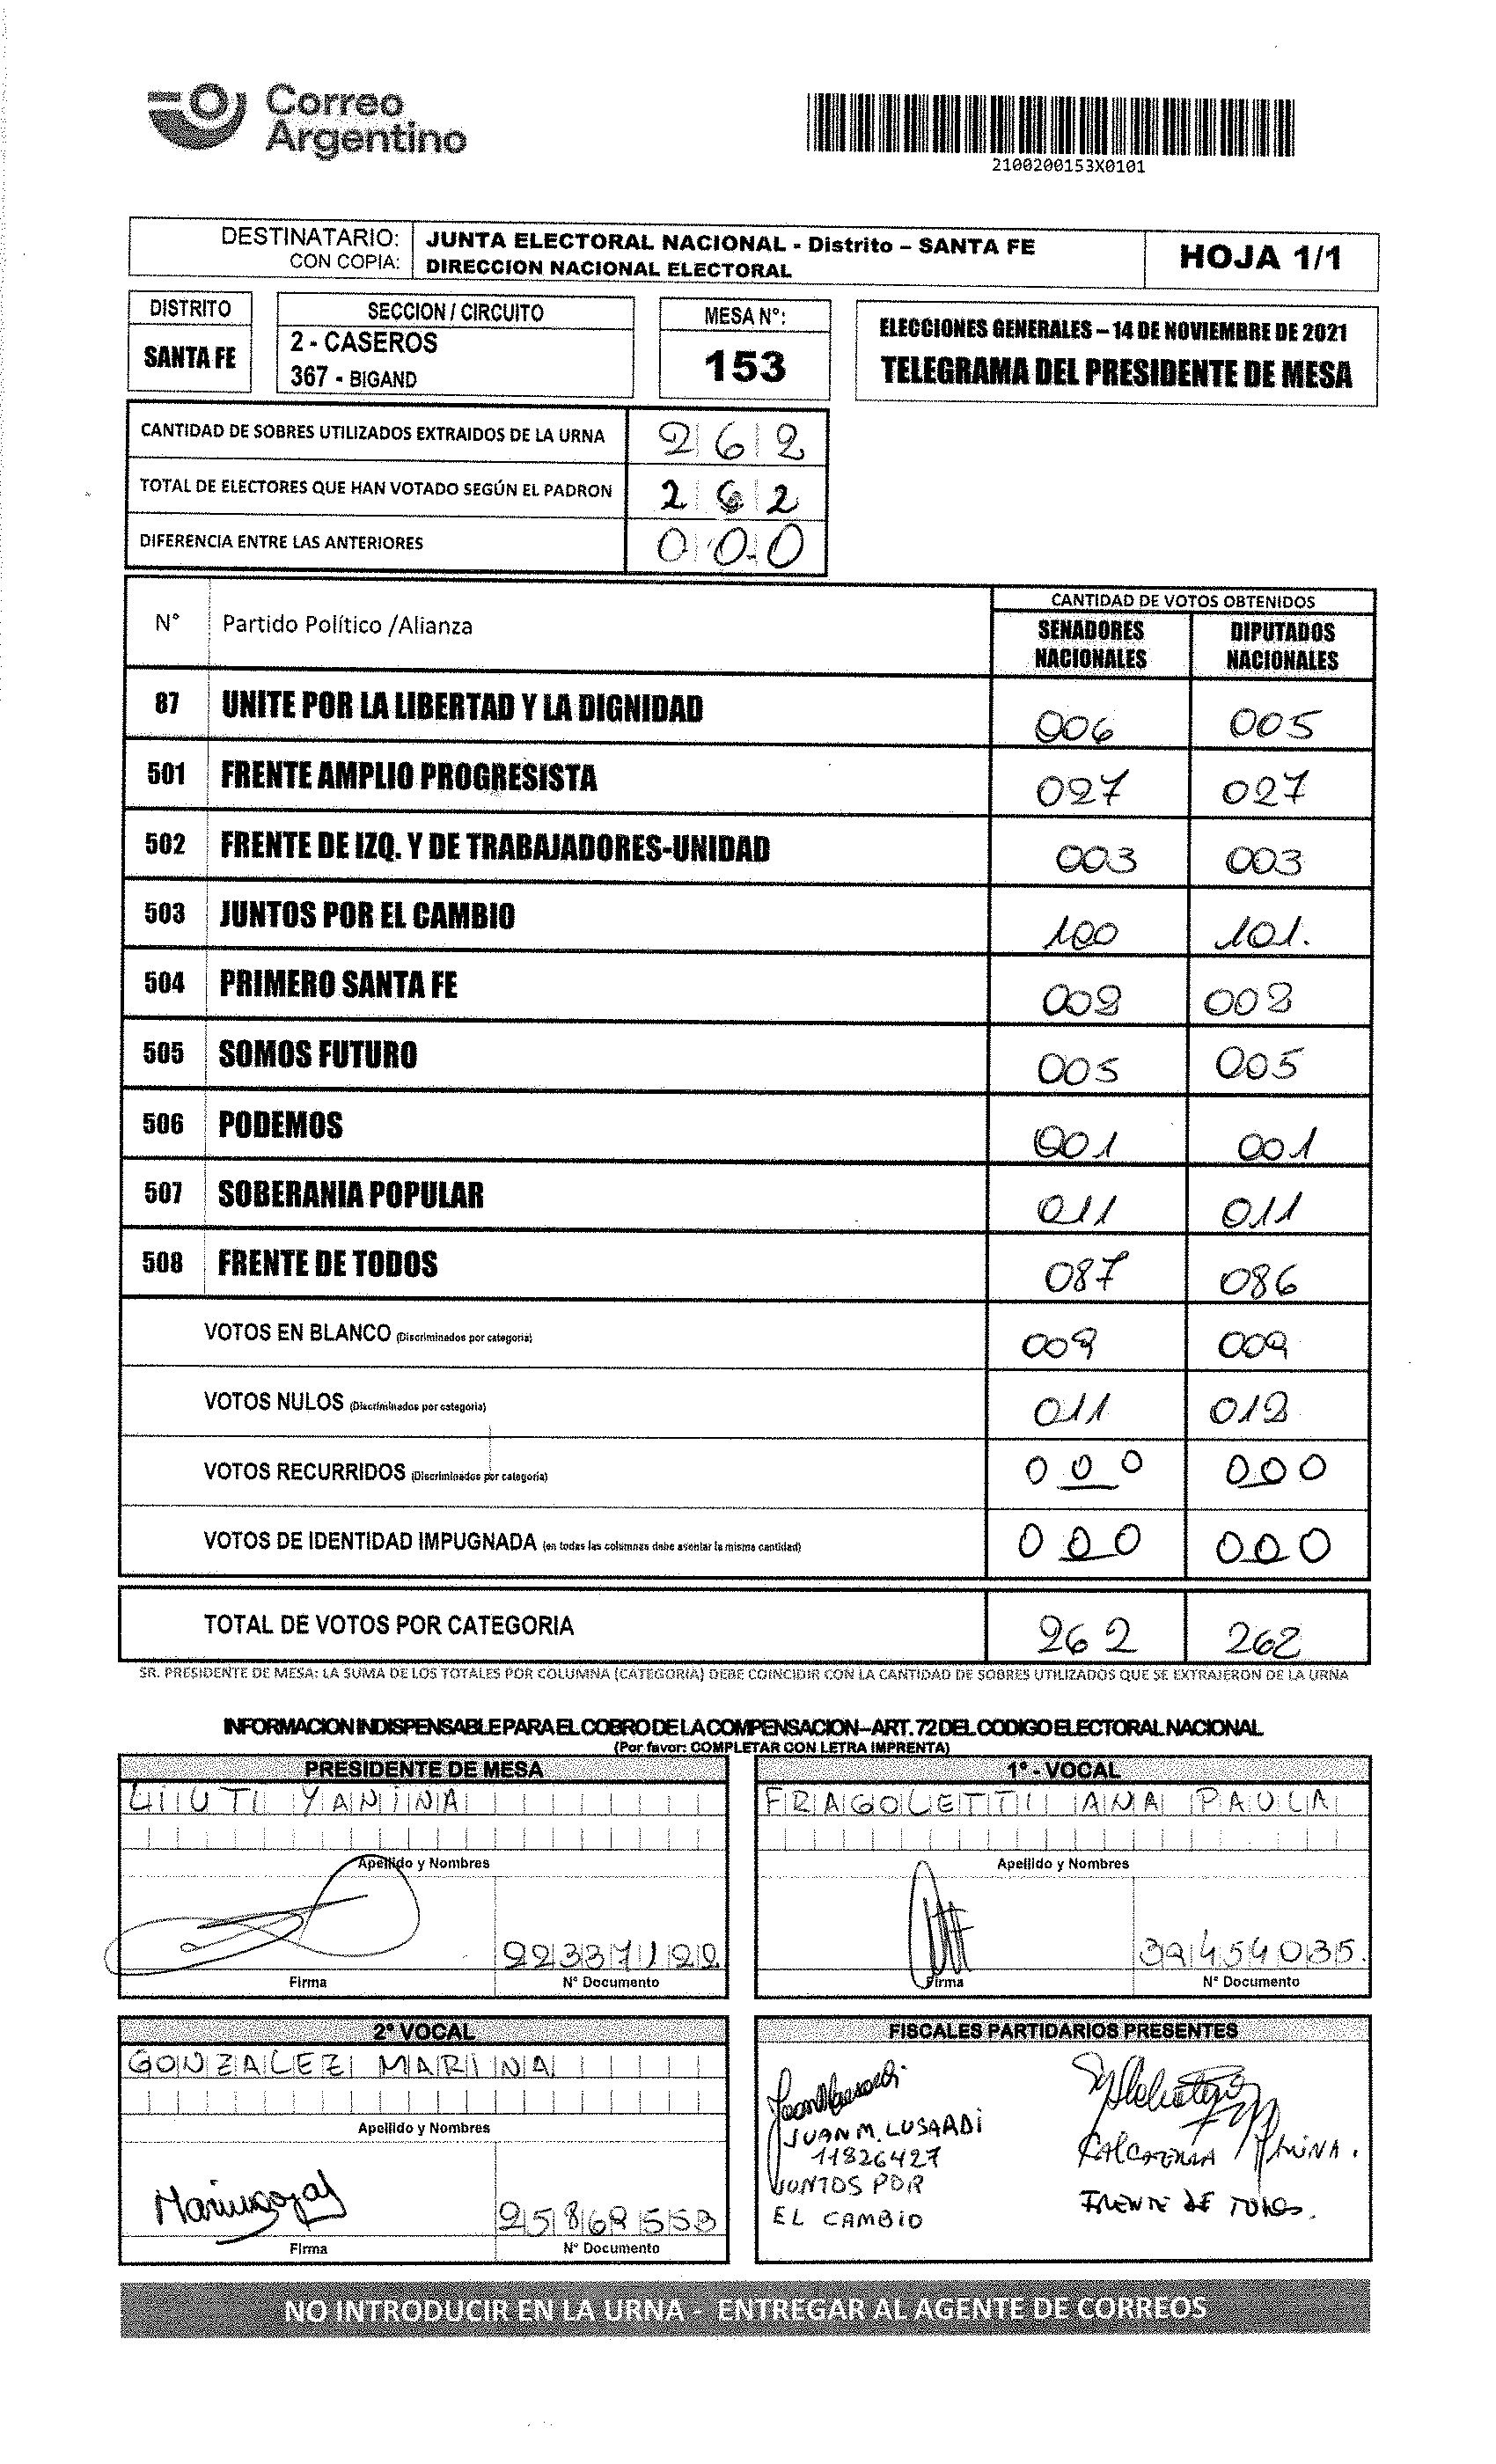
\includegraphics[height=0.8\textheight]{appendices/telegrama-numeros-juntos.jpg}

\section{Ejemplo de telegrama con caracteres distintos a números}
\label{anexo:telegrama-erroneo-caracteres-especiales}

El telegrama no utiliza únicamente dígitos numéricos en la cantidad de votos.

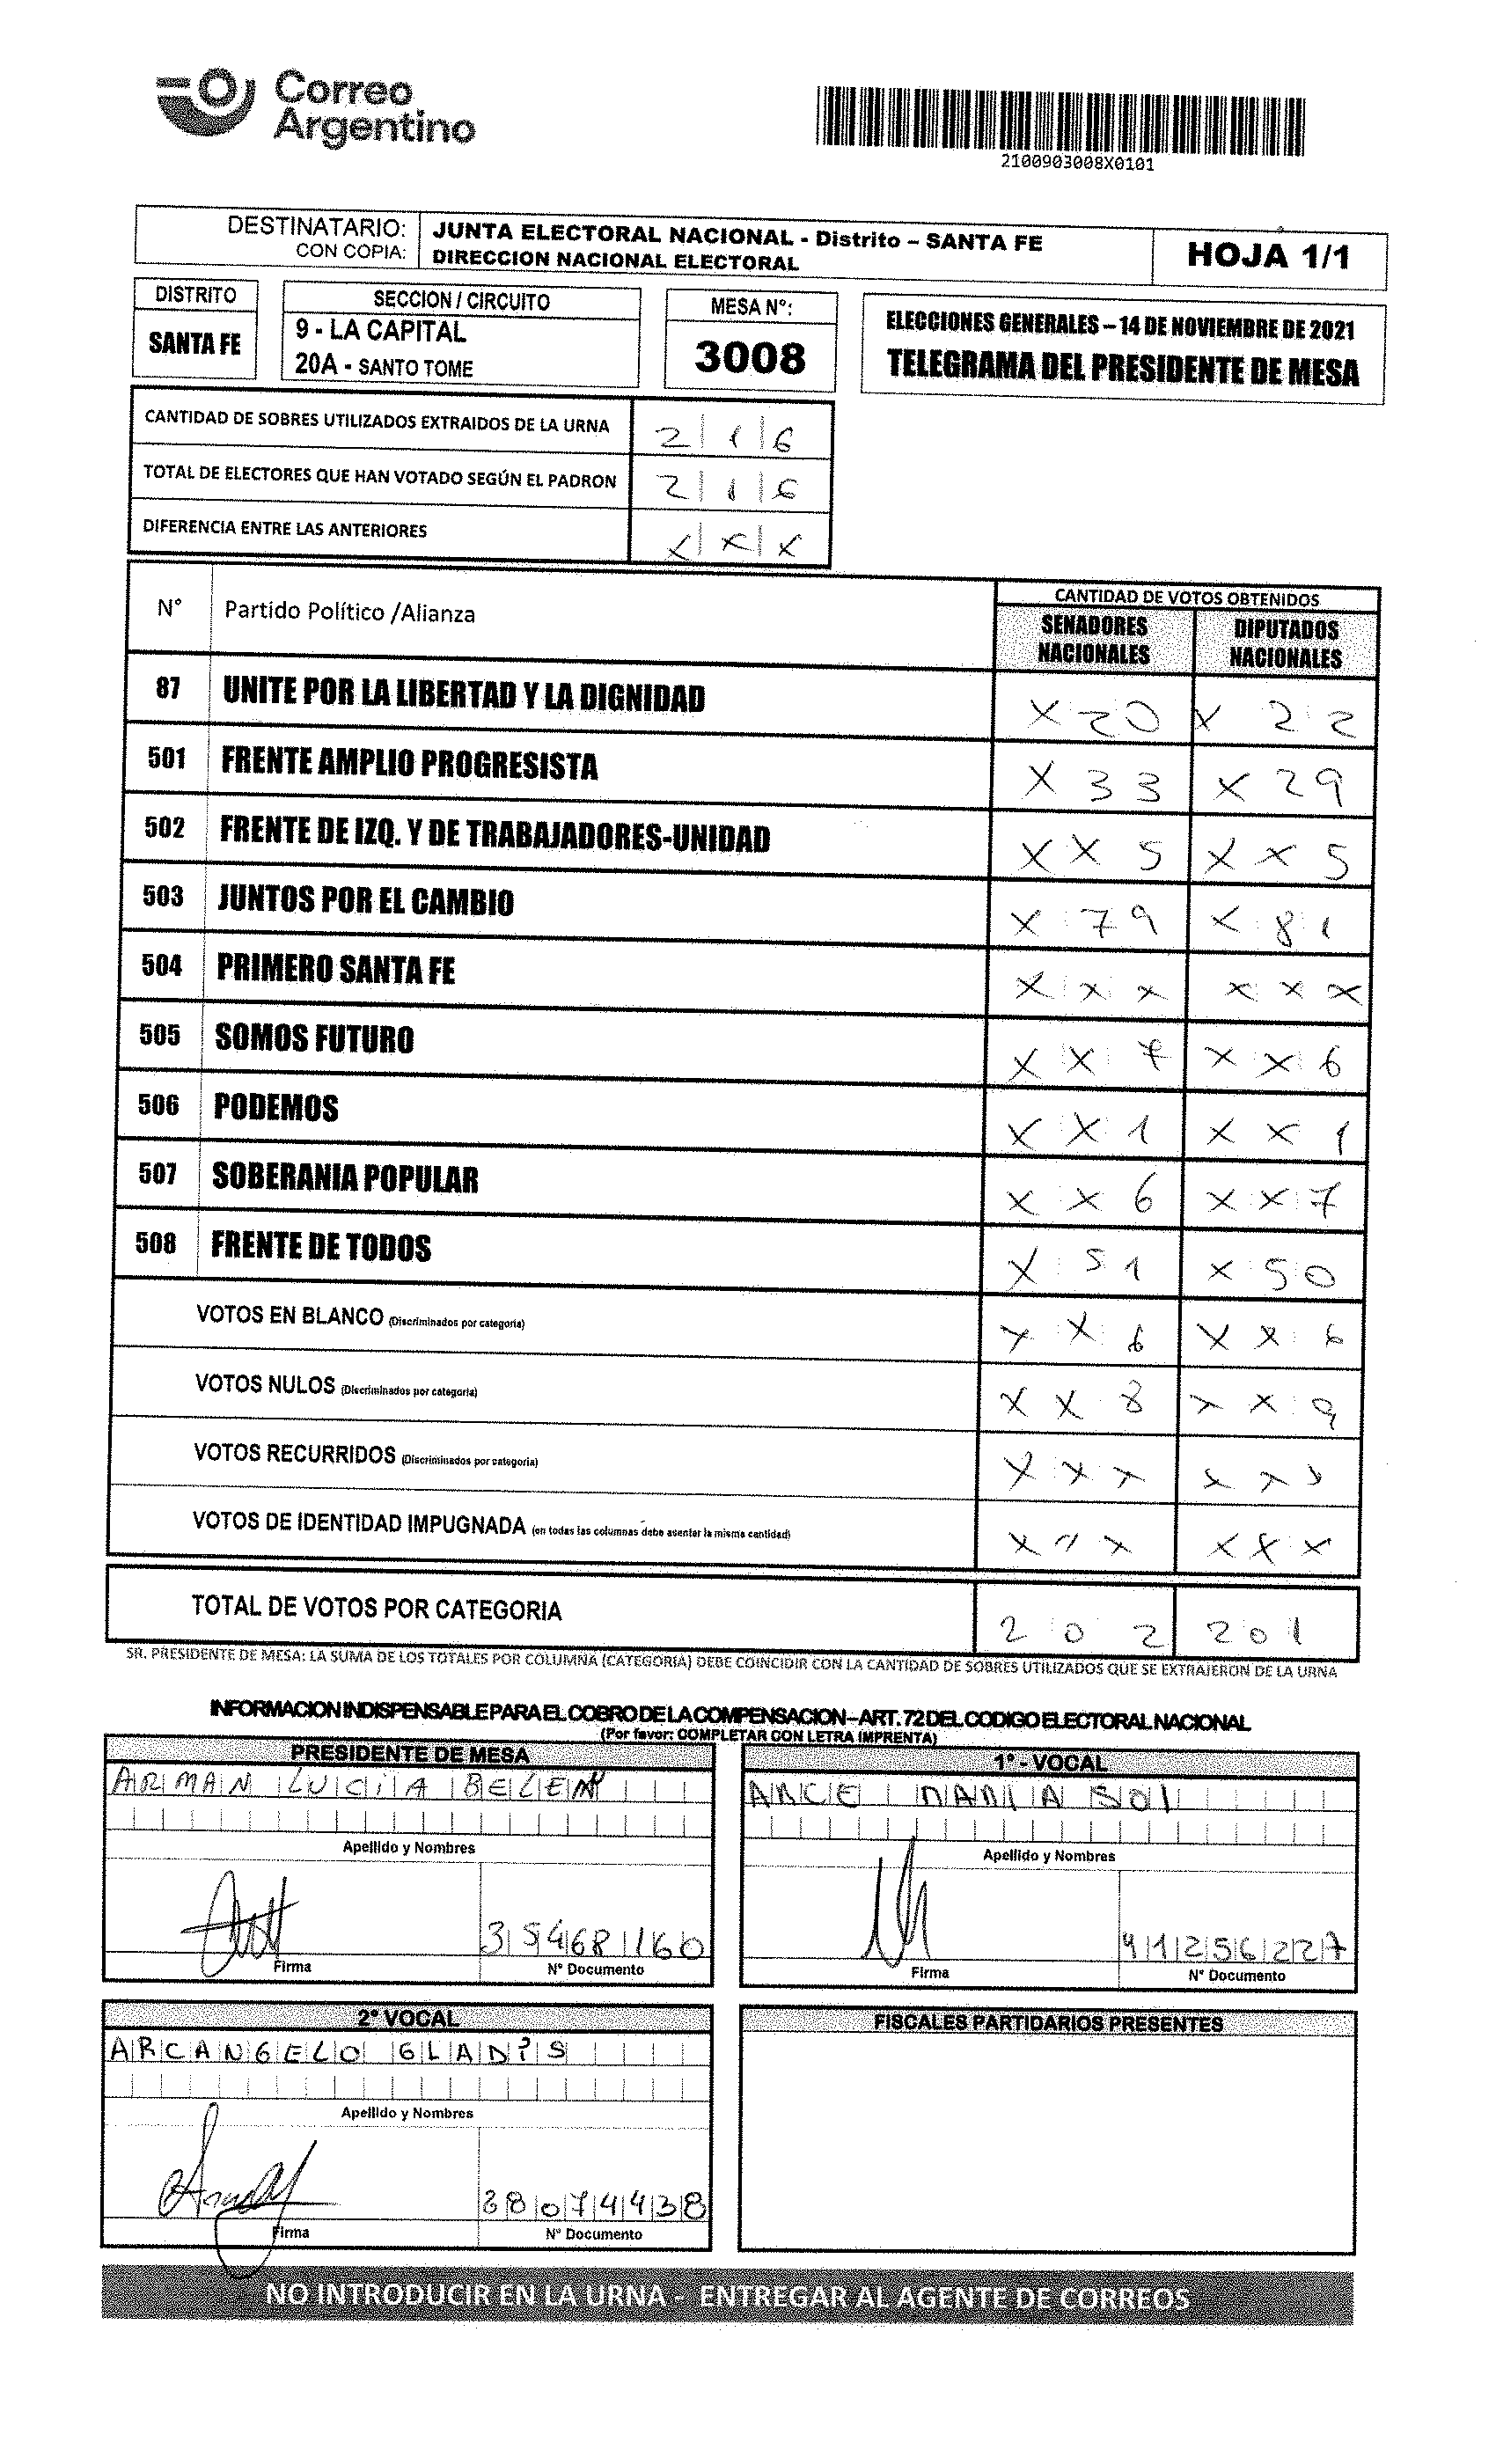
\includegraphics[height=0.8\textheight]{appendices/telegrama-erroneo-caracteres-especiales.png}

\section{Ejemplo de telegrama ceros a la izquierda de la cantidad de votos}
\label{anexo:telegrama-erroneo-muchos-ceros}

El telegrama posee ceros a la izquierda en la cantidad de votos, por lo que aumenta la probabilidad de predecir
erróneamente la cantidad de votos.

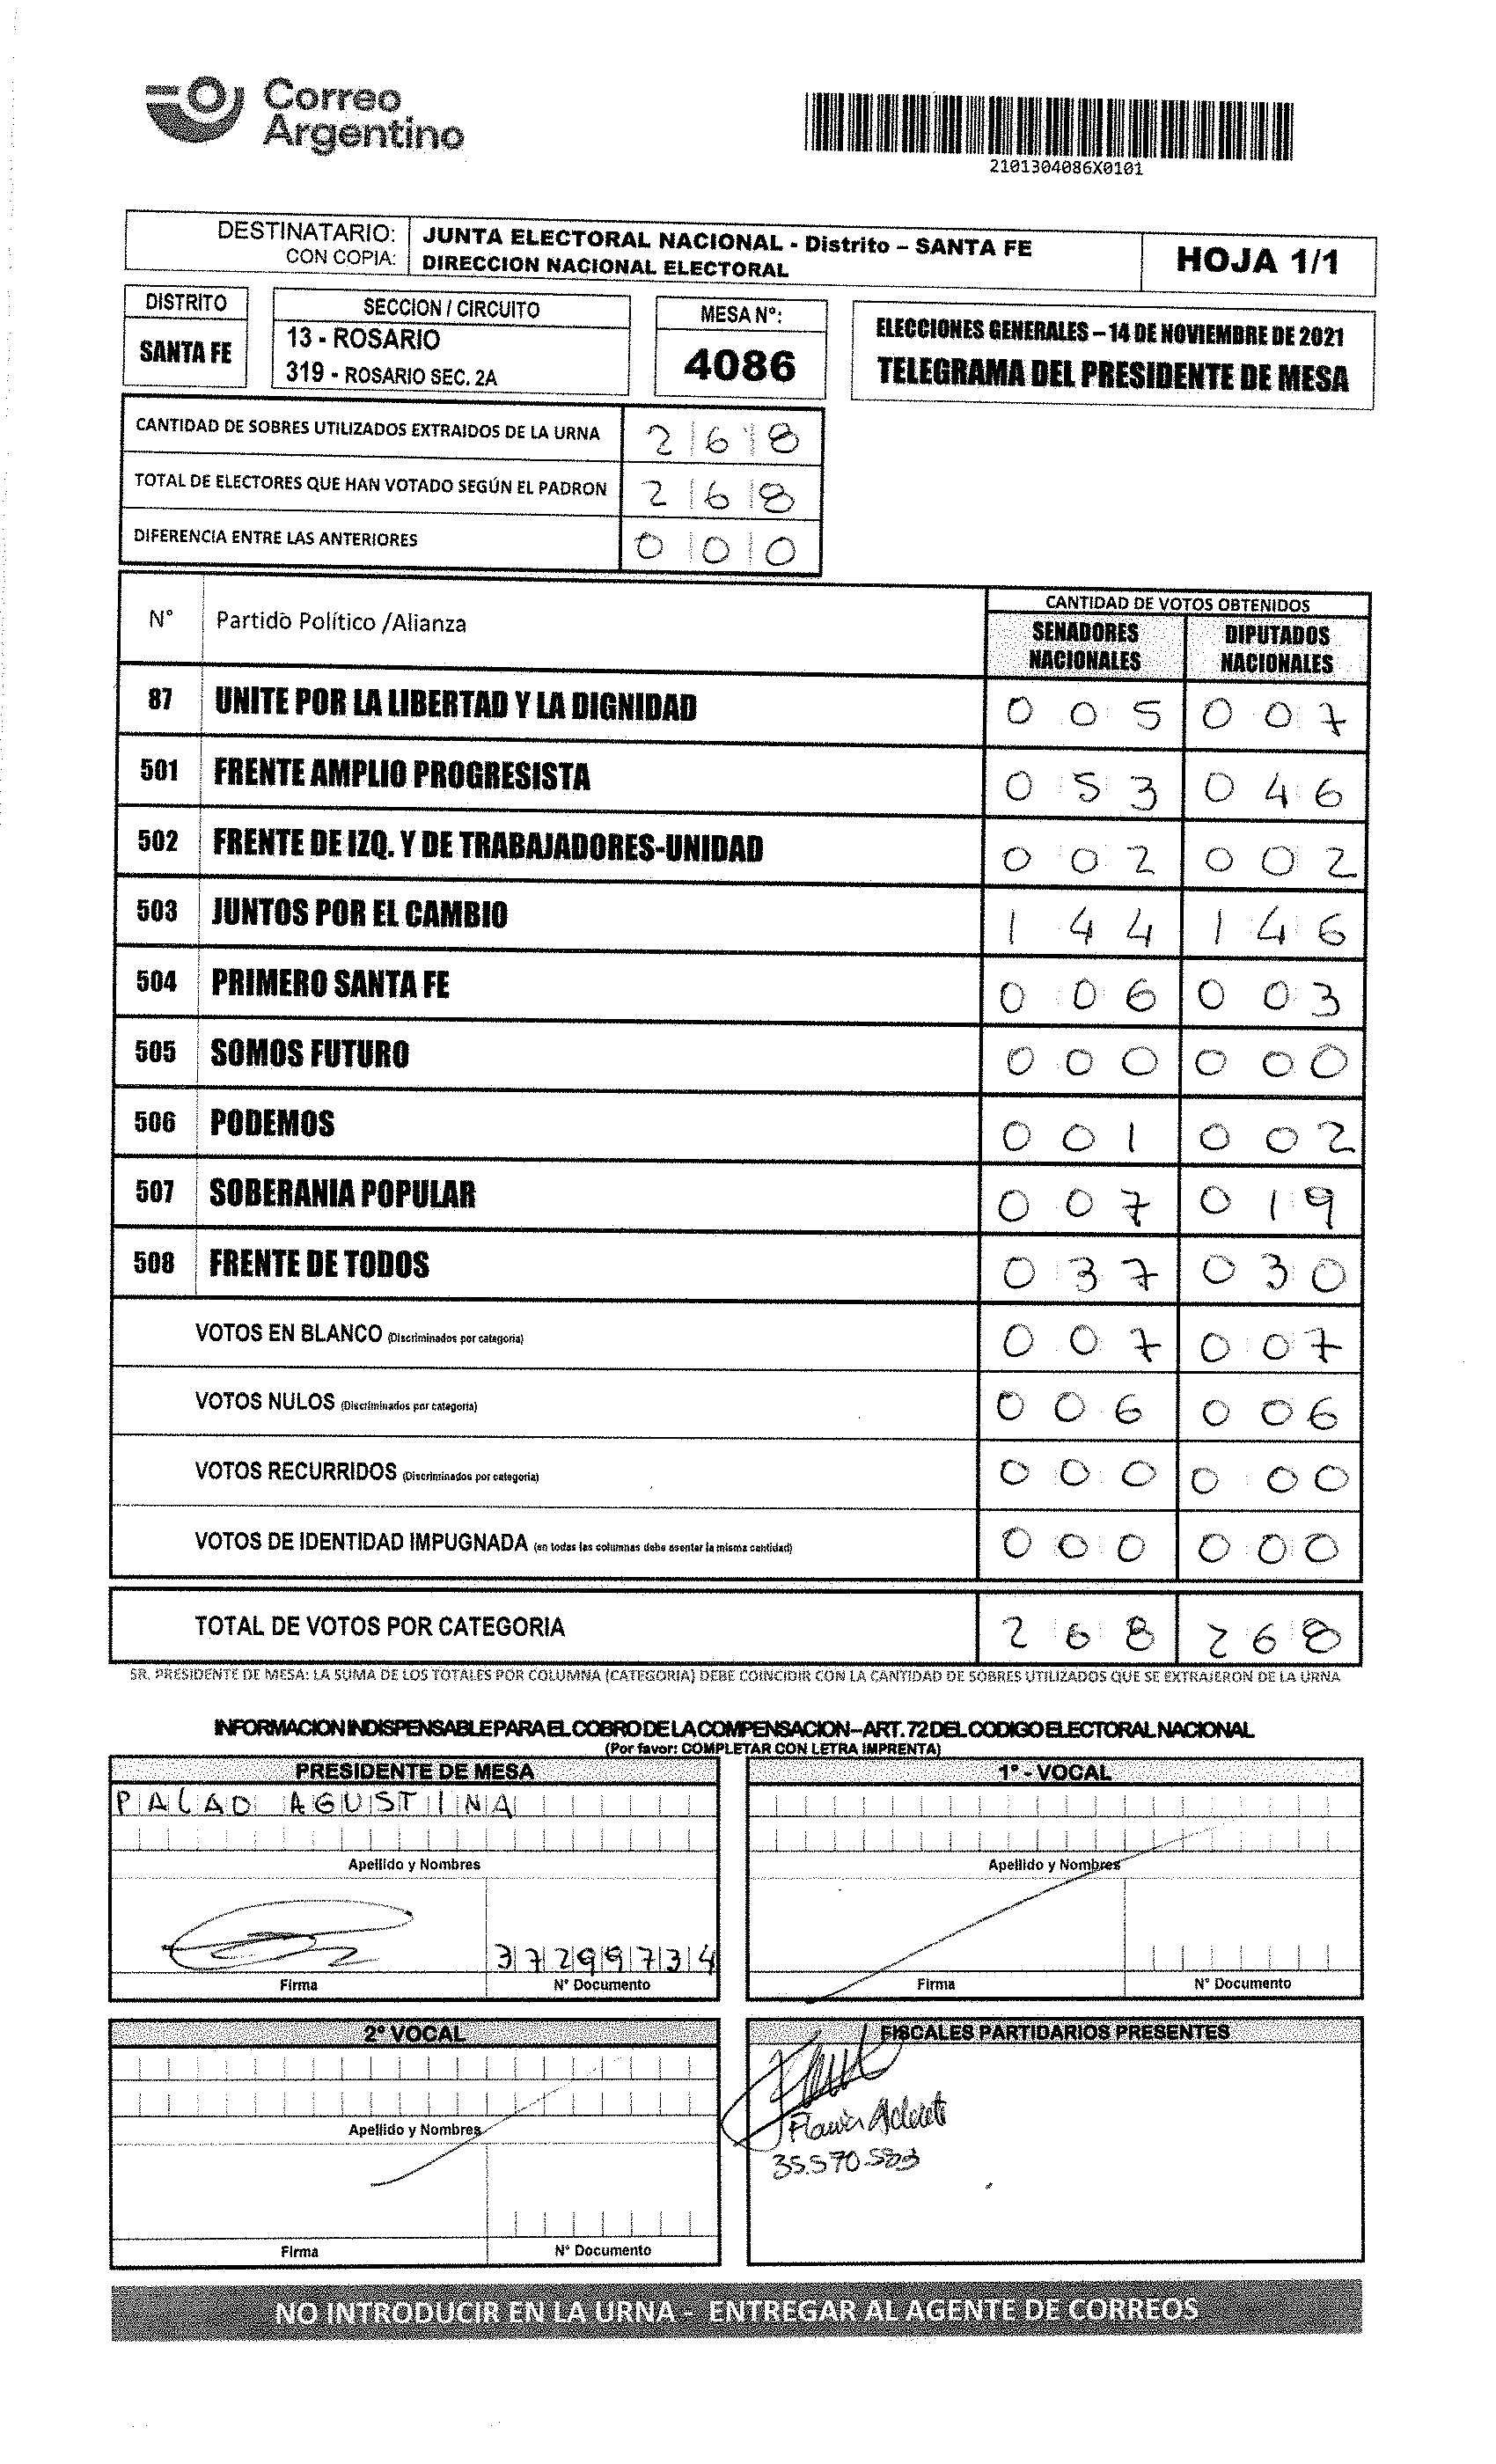
\includegraphics[height=0.8\textheight]{appendices/telegrama-erroneo-muchos-ceros.png}
